% !TEX root = main.tex
\chapter[head={The CKM angle $\gamma$},tocentry={The CKM angle $\symbfsf{\gamma}$}]{The CKM angle $\symbfsf{\gamma}$}
\label{ch:CKMAngleGamma}

As mentioned before overconstraining the triangle relations following from the unitarity of the matrix is a nice experimental self consistency check of the \ac{SM}.
The CKM angle $\gamma$ is one of five observables parametrising the CKM triangle described in \cref{eq:CKMtriangle}.
The current experimental constraints on this triangle are shown in \cref{fig:ckmtriangle}.
One can see that $\gamma$ is currently the least well known parameter.
Hence the more accurate determination of $\gamma$ is one of the main tasks of current research in the field of flavour physics.
This chapter is organised as follows: Firstly it is described how $\gamma$ can be accessed in section \cref{sec:accessGamma}, especially the determination using tree-level decays (\cref{sec:gamamInTrees}) and loop-processes (\cref{sec:gamamInLoops}) is emphasized, followed by the explanation how the decay mode \BdToDpi can be used to derive constraints $\gamma$ in \cref{sec:GammaInBd2Dpi}.

\begin{figure}[tbp]
	\centering
	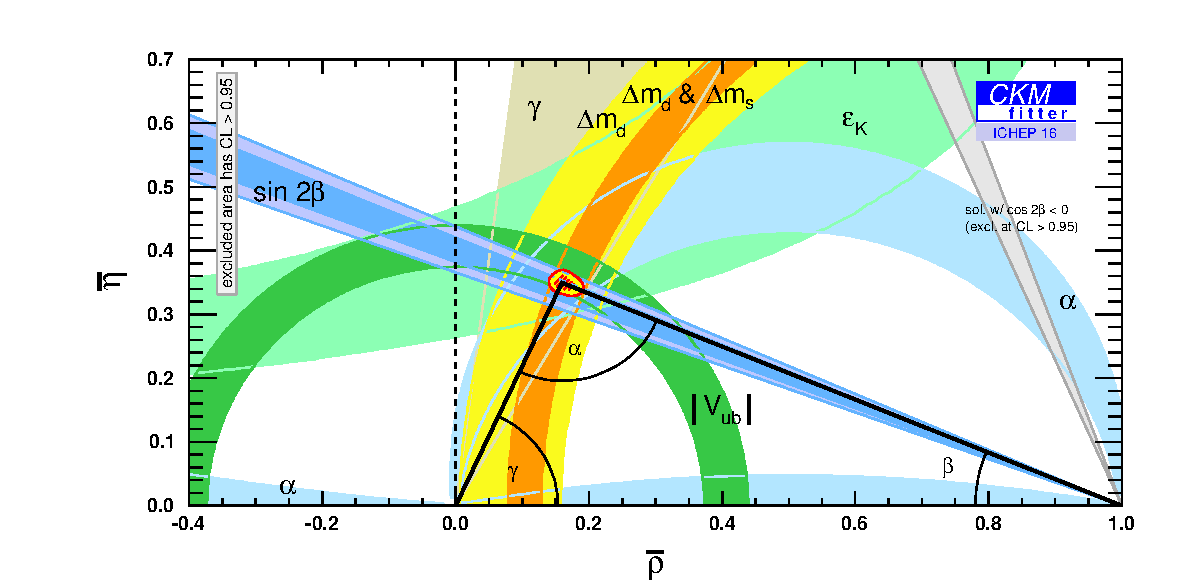
\includegraphics[width=0.8\textwidth]{04gamma/figs/CKMTriangle.pdf}
	\caption{CKM triangle in the complex plane.
	The coloured bands show the experimental constraints.
	The red hashed and the yellow area around the apex represents the currrent ucnertainties at \SI{68}{\percent} and \SI{95}{\percent} confidence level, respectively~\cite{CKMfitter2015}.}
	\label{fig:ckmtriangle}
\end{figure}

\section[head={Accessing the angle $\gamma$},tocentry={Accessing the angle $\gamma$}]{Accessing the angle $\symbfsf{\gamma}$}
\label{sec:accessGamma}

As mentioned above the angle $\gamma=\arg\left(-\Vud\Vcb\Vubst\Vcdst\right)$ is the least well know angle in the unitarity triangle.
It is proportional to the phase of the matrix element \Vub and can consequently be determined by exploiting interference effects between the Cabibbo favoured transitions from \bquark's to \cquark's and the Cabibbo suppressed $\bquark\to\uquark$ transitions.
Due to this in principle it can be measured using only tree-level decays.
However as $\gamma$ is the phase of the matrix element \Vub, decays in which it can be measured are highly suppressed and therefore the precision of those measurements taken individually do not yield a satisfactory precision.
Thus the strategy to measure it is not mainly driven by one single decay mode as it is for the angle $\beta$ which can be nicely measured in a time dependent analysis of \BdToJPsiKS, but by measuring it in various different decays modes and combine the results statistically.
As in the \B meson system two types of \CP violation are expected at a non-neglibile amount decays which show effects of either direct \CP violation or interference \CP violation are studied.
In \cref{sec:gammainChargedModes} methods for decays which suffer direct \CP violation as the $\Bu\to\Dz\Kp$ or the $\Bu\to\Dz\Kp\pip\pim$ as the GLW and the GGSZ method will be discussed.
To measuring \gamma in interference \CP violation on first glimpse the decay $\Bs\to\rho\KS$ seems to be nice.
As $\rho\KS$ is a \CP eigenstate only the parameter \Lf has to be calculated using the amplitudes
\begin{equation}
\begin{aligned}
\Af&=\left<\rho\KS\left|T\right|\Bs\right>=-\frac{1}{2q_{\kaon}}\left<\rho\Kzb\left|T\right|\Bs\right>=-\frac{1}{2q_{\kaon}}\Vubst\Vud\\
\Abarf&=\left<\rho\KS\left|T\right|\Bsb\right>=\frac{1}{2p_{\kaon}}\left<\rho\Kz\left|T\right|\Bsb\right>=\frac{1}{2p_{\kaon}}\Vub\Vudst
\end{aligned}
\end{equation}
where $q_{\kaon}$ and $p_{\kaon}$ are the same mixing parameters for the neutral kaon system as shwon in \cref{eq:qoverp} for the \B-meson system.
Using $\nicefrac{q_{\kaon}}{p_{\kaon}}=\nicefrac{\Vcsst\Vcd}{\Vcs\Vcdst}$ the parameter \Lf can be calculated as
\begin{equation}
\Lf=-\frac{q_{\kaon}}{p_{\kaon}}\frac{q}{p}\frac{\left<\rho\Kz\left|T\right|\Bsb\right>}{\left<\rho\Kzb\left|T\right|\Bs\right>}
=-\frac{\Vcsst\Vcd}{\Vcs\Vcdst}\frac{\Vtbst\Vts}{\Vtb\Vtsst}\frac{\Vub\Vudst}{\Vubst\Vud}.
\end{equation}
With the CKM matrix developed up to third order in the parameter $\lambda$ (see \cref{eq:CKMmatrix}) this simplifies to a pure phase
\begin{equation}
\Lf=e^{-2i\gamma}
\end{equation}
and could provide a good candidate to measure the CKM angle $\gamma$.

Though, up to date \CP violation has only been detected in the quark sector and therefore strong interactions are unavoidable.
This means that beside tree-level diagrams there are also gluonic penguins, what complicates most analysis as these diagrams usually carry a weak phase different from the one in the tree-level diagram.
Additionally the hadronic matrix elements cannot be calculated reliably, resulting in large uncertainties in the determination of the sides and angles of the unitarity triangle.
To understand the effect of an additional weak phase contributing, one can consider two weak phases contributing to the transitions $\Af$ and $\Abarf$:
\begin{equation}
\begin{aligned}
\Af&=A_1e^{i\left(\Phi_{A_1}+\delta_1\right)}+A_2e^{i\left(\Phi_{A_2}+\delta_2\right)}\\
\Abarf&=\eta_f\left[A_1e^{i\left(-\Phi_{A_1}+\delta_1\right)}+A_2e^{i\left(-\Phi_{A_2}+\delta_2\right)}\right]
\end{aligned}
\end{equation}
As shown in \cref{eq:qoverPPurePhase} the quantity $\nicefrac{q}{p}$ is a pure phase and hence one can write $\nicefrac{q}{p}=-e^{2i\Phi_\text{M}}$, what leads to
\begin{equation}
\Lf=-\eta_fe^{2i\Phi_\text{M}}\frac{ A_1 e^{i\left(-\Phi_{A_1}+\delta_1\right)} + A_2 e^{i\left(-\Phi_{A_2}+\delta_2\right)}}{A_1e^{i\left(\Phi_{A_1}+\delta_1\right)}+A_2e^{i\left(\Phi_{A_2}+\delta_2\right)}}
\end{equation}
The phases $\Phi_{A_1}$, $\Phi_{A_2}$ and $\Phi_\text{M}$ are not rephasing-invariant, but the relative phases $\Phi_1\equiv\Phi_{A_1}-\Phi_\text{M}$, $\Phi_1\equiv\Phi_{A_2}-\Phi_\text{M}$ and $\Delta=\delta_2-\delta_1$ can be measured. Therefore one finds
\begin{align}
\Lf&=-\eta_fe^{-2i\Phi_1}\frac{1+re^{i\left(\Delta-\Phi_2+\Phi_1\right)}}{1+re^{i\left(\Delta+\Phi_2-\Phi_1\right)}}\nonumber\\
&\approx-\eta_fe^{-2i\Phi_1}\left[1+2r\sin\Delta\sin\left(\Phi_2-\Phi_1\right)-2ir\cos\Delta\sin\left(\Phi_2-\Phi_1\right)\right],
\end{align}
where the approximation that $r=\nicefrac{A_2}{A_1}$ is small was used.

Now one finds, that in case a second penguin with a different weak phase from that of the tree-level diagram contributes the parameter and $r\neq0$, \Lf does not allow to measure a single weak phase. Though even in the case of vanishing final state interactions, \ie $\Delta=0$, \Lf can just be written as
\begin{equation}
\Lf=-\eta_fe^{-2i\left(\Phi_1-\delta_{\Phi_1}\right)}
\end{equation}
where $\delta_{\Phi_1}$ is defined by
\begin{equation}
\tan\left(\delta_{\Phi_1}\right)=\frac{r\sin\left(\Phi_1-\Phi_2\right)}{1+r\cos\left(\Phi_1-\Phi_2\right)}.
\end{equation}
In the case of $\Bs\to\rho\KS$ the $\rho$ in the finalstate has a \uquark\uquarkbar and a \dquark\dquarkbar component.
This means that alongside the spectator \squark-quark not only the tree level transition $\bquark\to\uquark\uquarkbar\dquarkbar$ but also the gluonic penguin transition $\bquark\to\dquark\dquarkbar\dquarkbar$ is possible (see \cref{fig:Bs2RhoKS}).
\begin{figure}[tbp]
	\centering
	\includestandalone{04gamma/figs/BsToRhoKS_Tree}
	\includestandalone{04gamma/figs/BsToRhoKS_Penguin}
	\caption{Tree-level diagram of $\Bs\to\rho\KS$ (left) and the dominantly contributing gluonic penguin (right). \cite{Ellis:2016jkw}.}
	\label{fig:Bs2RhoKS}
\end{figure}
For both diagrams the CKM-factor is $\propto A\lambda^3$, but the weak phases are $\gamma$ and $beta$ for the tree-level diagram and the penguin, respectively.

Due to this penguin pollution the angle $\gamma$ cannot be measured in interference \CP violation in a decay to a \CP eigenstate.
Instead decays into non-\CP-eigenstates as \BsToDsK and \BdToDpi are needed.
These require a study of both finalstates separately and are hence more demanding as \eg detection asymmetries between the finalstates need to be taken into account (see \cref{sec:cpvInBd2Dpi}).

\subsection[head={Determination of $\gamma$ in tree-level decays},tocentry={Determination of $\gamma$ in tree-level decays}]{Determination of $\symbfsf{\gamma}$ in tree-level decays}
\label{sec:gamamInTrees}
Here I'm going to write about the GLW and ADS methods and DsK and Dpi

\subsection[head={Determination of $\gamma$ in loop processes},tocentry={Determination of $\gamma$ in loop processes}]{Determination of $\symbfsf{\gamma}$ in loop processes}
\label{sec:gamamInLoops}
Read the fleischer paper and understand the experimental status

\subsection{Experimental precision}

\section[head={Measuring $\gamma$ in $\Bz\to\Dm\pip$},tocentry={Measuring $\gamma$ in $\Bz\to\Dm\pip$}]{Measuring $\symbfsf{\gamma}$ in $\symbfsf{\Bz\to\Dm\pip}$}
\label{sec:GammaInBd2Dpi}
